\documentclass[10pt,twocolumn]{article}
\usepackage[margin=16mm]{geometry}
\usepackage{graphicx,amsmath,amssymb,booktabs,xcolor}
\usepackage[T1]{fontenc}
\usepackage{times}
\usepackage[hidelinks,breaklinks]{hyperref}
\usepackage{url}\urlstyle{tt}
\usepackage{caption}\captionsetup{font=small,labelfont=bf}
\usepackage{dblfloatfix}   % allow full-width (figure*) floats at page bottom too
\usepackage{flafter}       % never place a float before its first reference
\usepackage{placeins}      % \FloatBarrier to flush floats before a section
% Relax float packing so figures cluster near their mentions
\renewcommand{\topfraction}{0.95}
\renewcommand{\bottomfraction}{0.95}
\renewcommand{\textfraction}{0.05}
\renewcommand{\floatpagefraction}{0.7}
\renewcommand{\dbltopfraction}{0.95}
\renewcommand{\dblfloatpagefraction}{0.7}
\setcounter{topnumber}{3}\setcounter{bottomnumber}{2}
\setcounter{totalnumber}{5}\setcounter{dbltopnumber}{3}
\setlength{\parindent}{1.2em}
\setlength{\columnsep}{7mm}
\pagestyle{plain}
\newcommand{\um}{\,\textmu m}

\begin{document}
\twocolumn[{%
  \centering
  {\LARGE\bfseries Path-Parameter ILC with a Learned Correction Layer\\[2pt]
   for High-Accuracy Industrial Robots\par}
  \vspace{6pt}{\large Pravin Oli\par}
  \vspace{3pt}{\small Erasmus Mundus Joint Master in Intelligent Field Robotics
   Systems (IFROS)\\[1pt]
   Universitat de Girona, Spain \;$\cdot$\; E\"otv\"os Lor\'and University, Hungary\par}
  \vspace{3pt}{\small\texttt{pravin.oli.08@gmail.com}\par}
  \vspace{10pt}
  \begin{minipage}{0.86\textwidth}
  \small\textbf{Abstract}---The absolute accuracy of industrial robots is limited
  by unmodeled \emph{drivetrain error}: joint elasticity, gear transmission error,
  friction, backlash and thermal drift. A recent path-parameter iterative learning
  controller (ILC) cancels this error but relies on an external laser tracker to
  learn and leaves several problems open. We re-implement that ILC faithfully on a
  simulated KUKA iiwa14 whose every axis is modeled as a two-mass flexible joint,
  and address three of those open problems: (i) the error is self-learned from an
  integrated \emph{joint-side (output) encoder} rather than a laser tracker;
  (ii) a small learned model generalizes the correction to an \emph{unseen} path
  with zero trials; and (iii) a temperature-aware layer compensates a
  non-repetitive thermal drift that a fixed ILC table cannot. The ILC reduces the
  Cartesian tool error by ${\sim}32\times$ (to ${\approx}1$\,mm), the learned layer
  recovers near-converged accuracy on a new path instantly, and the thermal layer
  matches an oracle re-learn. We are explicit about what the simulation does and
  does not establish.
  \end{minipage}\vspace{14pt}
}]

\begin{figure}[t]
  \centering
  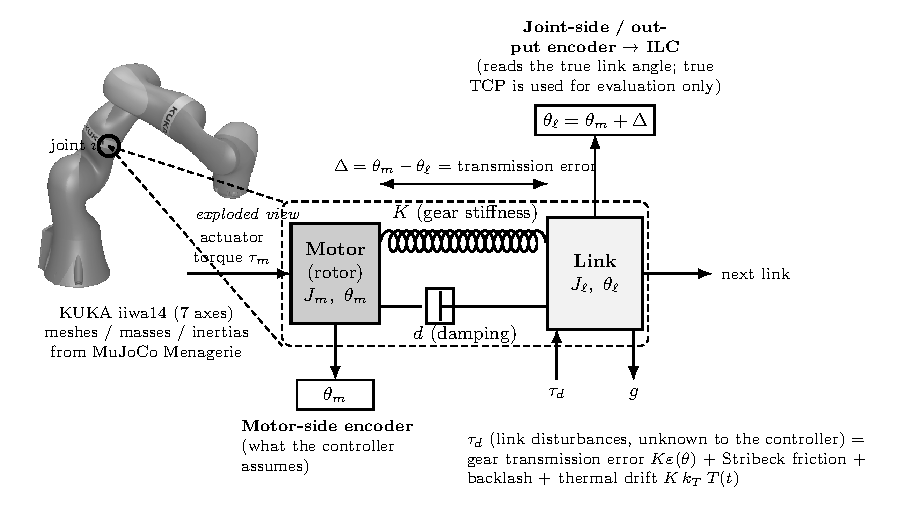
\includegraphics[width=\columnwidth]{model_schematic.pdf}
  \caption{Flexible-joint drivetrain model. Every axis of the real iiwa14 is a
  two-mass system: a motor inertia $J_m$ and a link inertia $J_\ell$ joined by a
  torsional spring $K$ and damper $d$. The controller plans on the rigid model
  ($\theta_\ell{=}\theta_m$); the link deflects, so $\Delta=\theta_m-\theta_\ell$
  is a real transmission error. The link also receives a disturbance torque
  $\tau_d$ (transmission error, friction, backlash, thermal drift), unknown to the
  controller. The \emph{joint-side / output} encoder reads the true link angle and
  feeds the ILC; the true Cartesian tool position is used only for evaluation.}
  \label{fig:model}
\end{figure}

\section{Introduction}
Industrial manipulators are highly \emph{repeatable} but their \emph{absolute}
accuracy is limited by effects a rigid kinematic model ignores: joint elasticity,
gear and cycloidal \emph{transmission error}, Stribeck friction, backlash, and
slow thermal drift~\cite{schwegel2024,litak2003}. Iterative learning control
(ILC) suits such \emph{repeatable} errors because it improves a feedforward
correction over repetitions of the same task~\cite{bristow2006}.

Schwegel and Kugi~\cite{schwegel2024} proposed a \emph{path-parameter} ILC that
indexes the learned correction by arc length $\lambda\in[0,1]$ rather than time,
so one table transfers across execution speeds; on a real 6-axis robot it reached
${\approx}95\%$ error reduction in two trials. However, it uses an external
\emph{laser tracker} to learn, and its conclusion lists four open problems:
speed-variation performance, contact tasks, a \emph{model-based learning filter},
and \emph{generalizing} the learned correction to different paths.

This paper re-implements that ILC and targets three open problems on a simulated,
physically detailed KUKA iiwa14. Contributions: (1) the drivetrain error is
self-learned from an \emph{integrated joint-side encoder} instead of a laser
tracker; (2) a small learned model predicts the correction for an \emph{unseen}
path with zero additional trials; and (3) a temperature-aware layer compensates a
non-repetitive thermal drift that a frozen ILC table cannot.

\section{Flexible-Joint Robot Model}\label{sec:model}
We use the real iiwa14 (meshes, masses, inertias from the MuJoCo
Menagerie~\cite{menagerie}) in MuJoCo~\cite{mujoco}, and turn every hinge into a
\emph{two-mass flexible joint}~\cite{spong1987} (Fig.~\ref{fig:model}): an actuated
motor degree of freedom $\theta_m$ and a passive link degree of freedom
$\theta_\ell$ coupled by a torsional spring $K$ and damper $d$. Per axis, $K$ ranges $18000{\to}3000$\,Nm/rad
and $d$ ranges $50{\to}8$\,Nms/rad from base to wrist, giving structural natural
frequencies $f_n\approx 10$--$195$\,Hz. Each axis therefore obeys a coupled
two-mass equation of motion,
\begin{equation}
J_m\ddot\theta_m = \tau_m - K\Delta - d\dot\Delta,\qquad
J_\ell\ddot\theta_\ell = K\Delta + d\dot\Delta - \tau_d,
\label{eq:eom}
\end{equation}
where $\tau_m$ is the commanded motor torque, $\Delta=\theta_m-\theta_\ell$ is the
elastic deflection, and $\tau_d$ is the link-side disturbance defined below. The
free torsional mode of this pair sits at $f_n=\tfrac{1}{2\pi}\sqrt{K/J_\ell}$,
which marks where structural \emph{vibration}---rather than the repeatable,
position-locked error the ILC targets---begins to dominate, and hence sets the
frequency above which the learning filter must roll off.

The controller plans on the \emph{rigid} model and never sees the springs, so the
link lags the motor by an unknown deflection $\Delta=\theta_m-\theta_\ell$. On top
of this, the link receives a disturbance torque
\begin{equation}
\tau_d = \underbrace{K\,\varepsilon(\theta)}_{\text{transmission}}
       + \tau_{f}(\dot\theta) + \tau_{\text{bl}}(\theta)
       + \underbrace{K\,k_T\,T(t)}_{\text{thermal}},
\label{eq:dist}
\end{equation}
with an angle-periodic gear error
$\varepsilon(\theta)=\sum_k a_k\sin(n_k\theta+\phi_k)$ ($0.3$--$0.8$\,mrad,
$n_k=13$--$37$ cyc/rev), Stribeck friction~\cite{armstrong1994}
$\tau_f=\big(F_c+(F_s{-}F_c)e^{-(\dot\theta/v_s)^2}\big)\operatorname{sign}(\dot\theta)$
($F_s/F_c=1.7$), a backlash dead-zone $\tau_{\text{bl}}$, and a slow thermal
offset whose temperature $T(t)$ is heated by friction and is therefore
\emph{non-repetitive}. None of these is given to the controller; the ILC must
discover the correction from the joint-side encoder alone.

\section{Path-ILC and the Learned Correction Layer}\label{sec:method}
\textbf{Path-parameter ILC.} Following~\cite{schwegel2024}, the correction is a
table $u[\lambda]$ indexed by the path parameter. After trial $i{-}1$ the update
at each index is the proportional--derivative law
\begin{equation}
\alpha_i[\lambda] = u_{i-1}[\lambda] + K_p\,e_q[\lambda] + K_d\,\dot e_q[\lambda],
\label{eq:pd}
\end{equation}
where $e_q=q_r-\theta_\ell$ is the joint error from the output encoder. A Gaussian
\emph{Q-filter} smooths the update along the path,
\begin{equation}
u_i = Q * \alpha_i,\qquad \sigma=\frac{\sqrt{\ln 2}}{2\pi f},
\label{eq:q}
\end{equation}
so non-repetitive, high-frequency content (e.g.\ encoder noise) is not learned. We
use the paper's gains $K_p{=}1$, $K_d{=}0.01$ and cutoff $f{=}5$\,Hz---an order of
magnitude below the slowest structural mode of \eqref{eq:eom} ($f_n\!\approx\!10$\,Hz),
so the table captures the repeatable, position-locked deflection while rejecting
joint vibration and sensor noise. Indexing by $\lambda$ rather than time
decouples the correction from execution speed: the same table is replayed against
arc length, so a slower or faster traversal reads out the identical feedforward.
The motor command is $q_r+u[\lambda]$ (Fig.~\ref{fig:loop}).

\textbf{Learned correction layer.} Classical ILC must re-run trials on \emph{each}
new path or operating point---impractical when the workpiece shifts slightly
between cycles, or when the robot warms over a shift. We instead treat the
converged correction as a function of \emph{context} and learn it offline. A
compact multilayer perceptron---two hidden layers of $256$ units with ReLU
activations (Fig.~\ref{fig:net})---maps a low-dimensional descriptor of the
desired path geometry to the full table $u[\lambda]$, and is trained by Adam on a
mean-squared loss; for the thermal study a temperature-indexed linear model plays
the same role. Crucially, every training target is an ILC table obtained the hard
way---by actually running trials on the MuJoCo plant for that context---and the
test context is held out, so the reported number is what the \emph{predicted}
feedforward achieves on the real plant for a path or thermal state the model never
saw. The contribution is this architecture: a context-adaptive learned layer
sitting on top of a classical, well-understood ILC, not a black box replacing it.

\begin{figure}[ht]
  \centering
  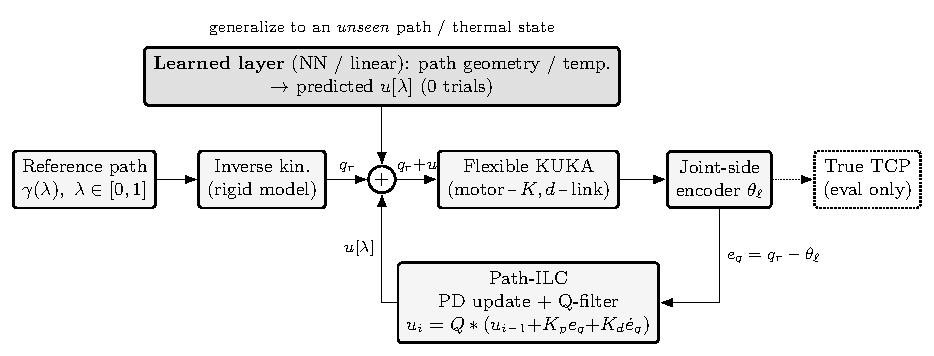
\includegraphics[width=\columnwidth]{method_loop.pdf}
  \caption{Control structure. The path-ILC learns $u[\lambda]$ from the joint-side
  encoder error; the learned layer predicts $u[\lambda]$ for an unseen path or thermal
  state with zero trials. The true TCP is used only for evaluation.}
  \label{fig:loop}
\end{figure}

\begin{figure}[ht]
  \centering
  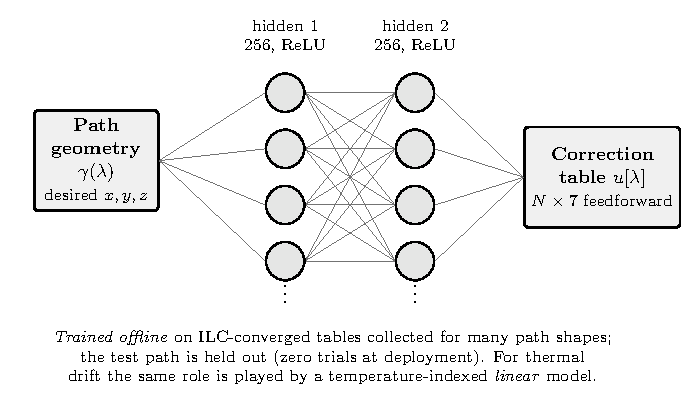
\includegraphics[width=\columnwidth]{network_architecture.pdf}
  \caption{Learned correction layer. A small multilayer perceptron maps the
  desired path geometry $\gamma(\lambda)$ to the entire feedforward table
  $u[\lambda]$ in one shot; it is trained offline on ILC-converged tables gathered
  for many path shapes, and the test path is held out so zero trials are run at
  deployment. The thermal variant replaces the network with a temperature-indexed
  linear model.}
  \label{fig:net}
\end{figure}

\section{Experimental Results}\label{sec:results}
All errors are Cartesian RMS at the tool tip, evaluated against the true
forward-kinematic TCP, which the controller never uses for learning. Each path is
sampled at $N{=}200$ arc-length points, every condition runs a handful of ILC
trials, and all runs are seeded, so each figure is regenerated end to end by a
single command. Table~\ref{tab:res} summarizes the headline experiments
(Fig.~\ref{fig:headline}), under the realistic repeatable disturbances of
\eqref{eq:dist}.

\begin{table}[t]
\centering\small
\caption{Headline results (Cartesian RMS at the tool tip).}
\label{tab:res}
\begin{tabular}{@{}ll@{}}
\toprule
Experiment & Result \\
\midrule
Convergence (output encoder only) & $34156\to1061\um$ (${\sim}32\times$)\\
Speed transfer (trained speed)    & ${\approx}997\um$ (partial elsewhere)\\
Path transfer (no learned layer)  & $42016\to14111\to1663\um$\\
\textbf{NN, unseen path, 0 tr.}& $34594\to5736\to\mathbf{1461\um}$\\
Contact task (${\sim}108$\,N press) & $18065\to1055\um$ (${\sim}17\times$)\\
\textbf{Learned, unseen thermal, 0 tr.}& frozen $4508\to\mathbf{988}\approx$ oracle $1050\um$\\
\bottomrule
\end{tabular}
\end{table}

\begin{figure*}[t]
  \centering
  \begin{minipage}{0.32\textwidth}\centering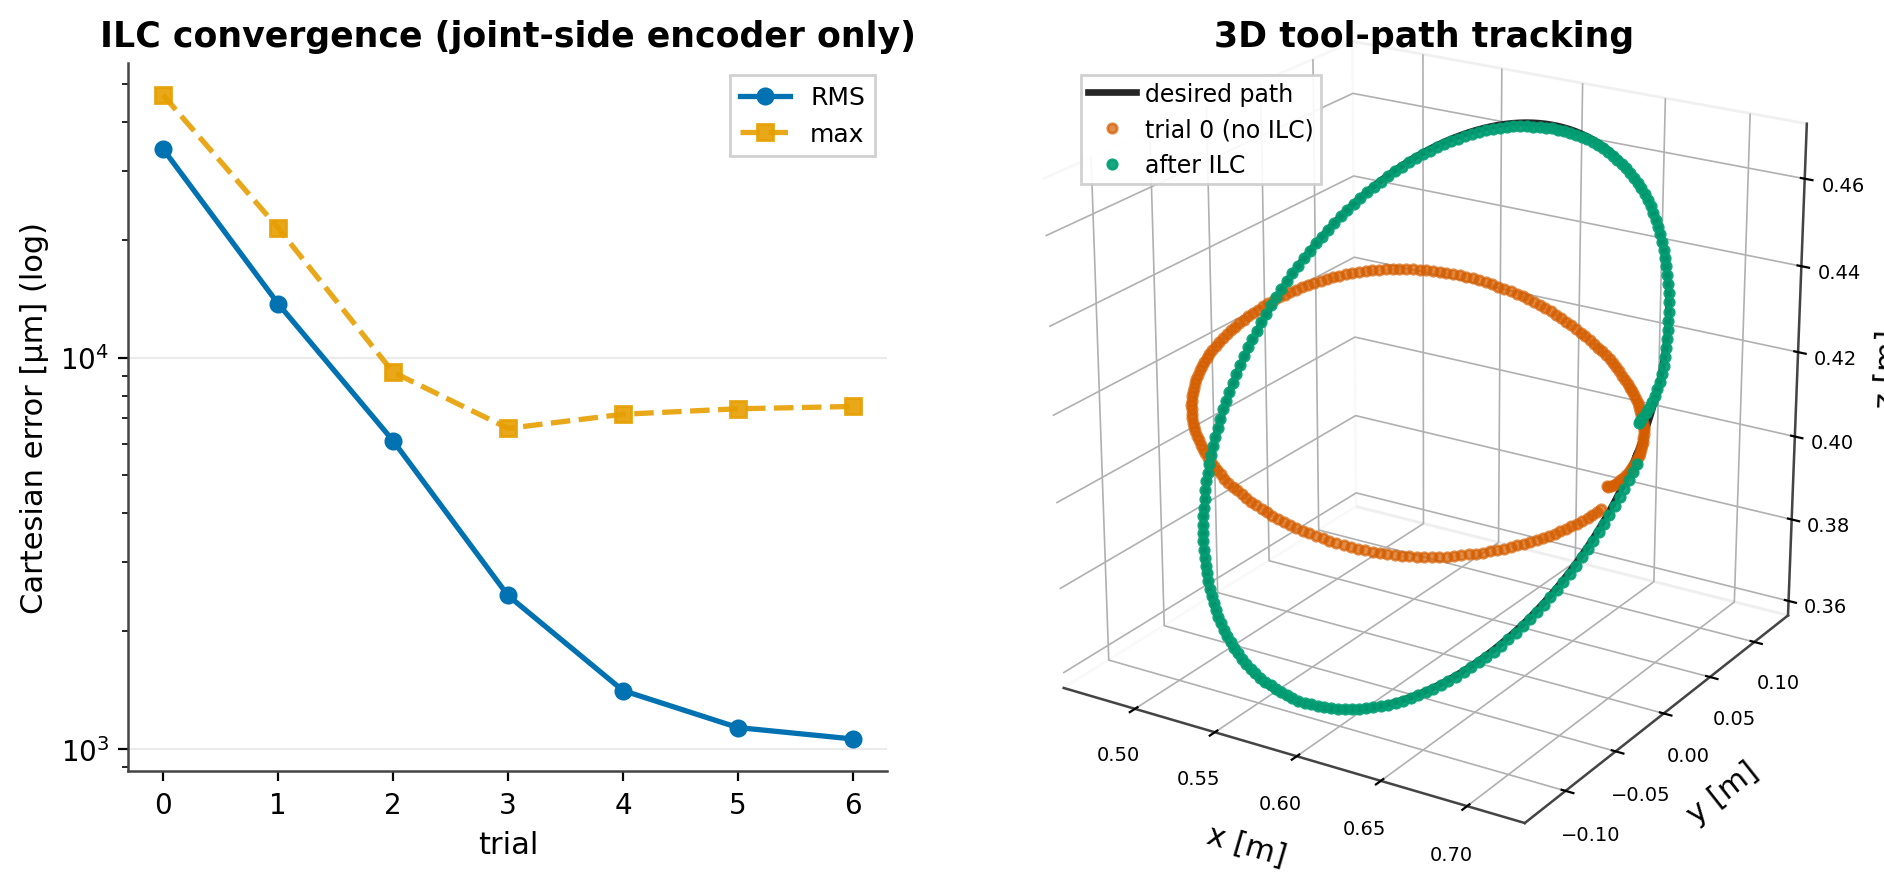
\includegraphics[width=\linewidth]{../outputs/kuka_convergence.png}\\{\footnotesize (a) convergence, encoder only}\end{minipage}\hfill
  \begin{minipage}{0.32\textwidth}\centering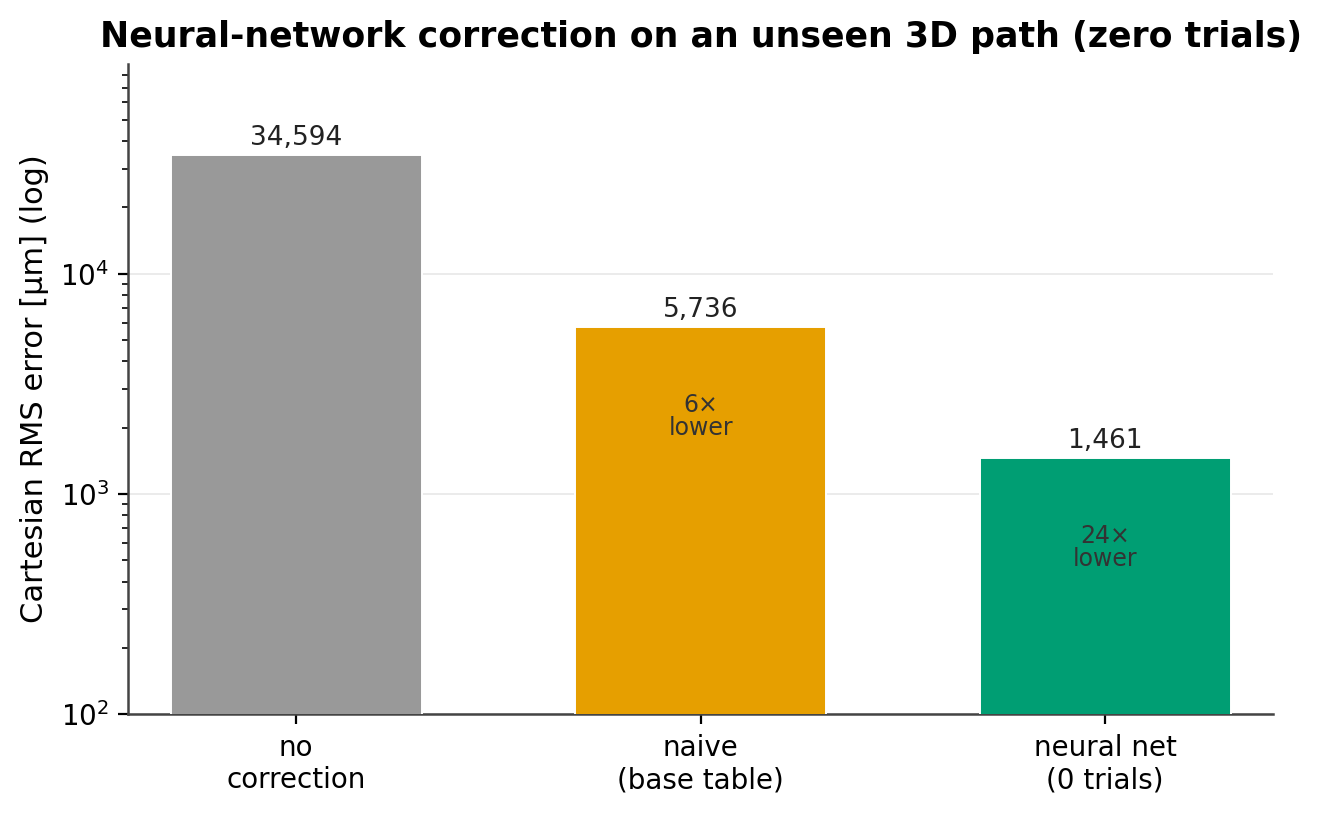
\includegraphics[width=\linewidth]{../outputs/kuka_nn_path_transfer.png}\\{\footnotesize (b) neural net, unseen path}\end{minipage}\hfill
  \begin{minipage}{0.32\textwidth}\centering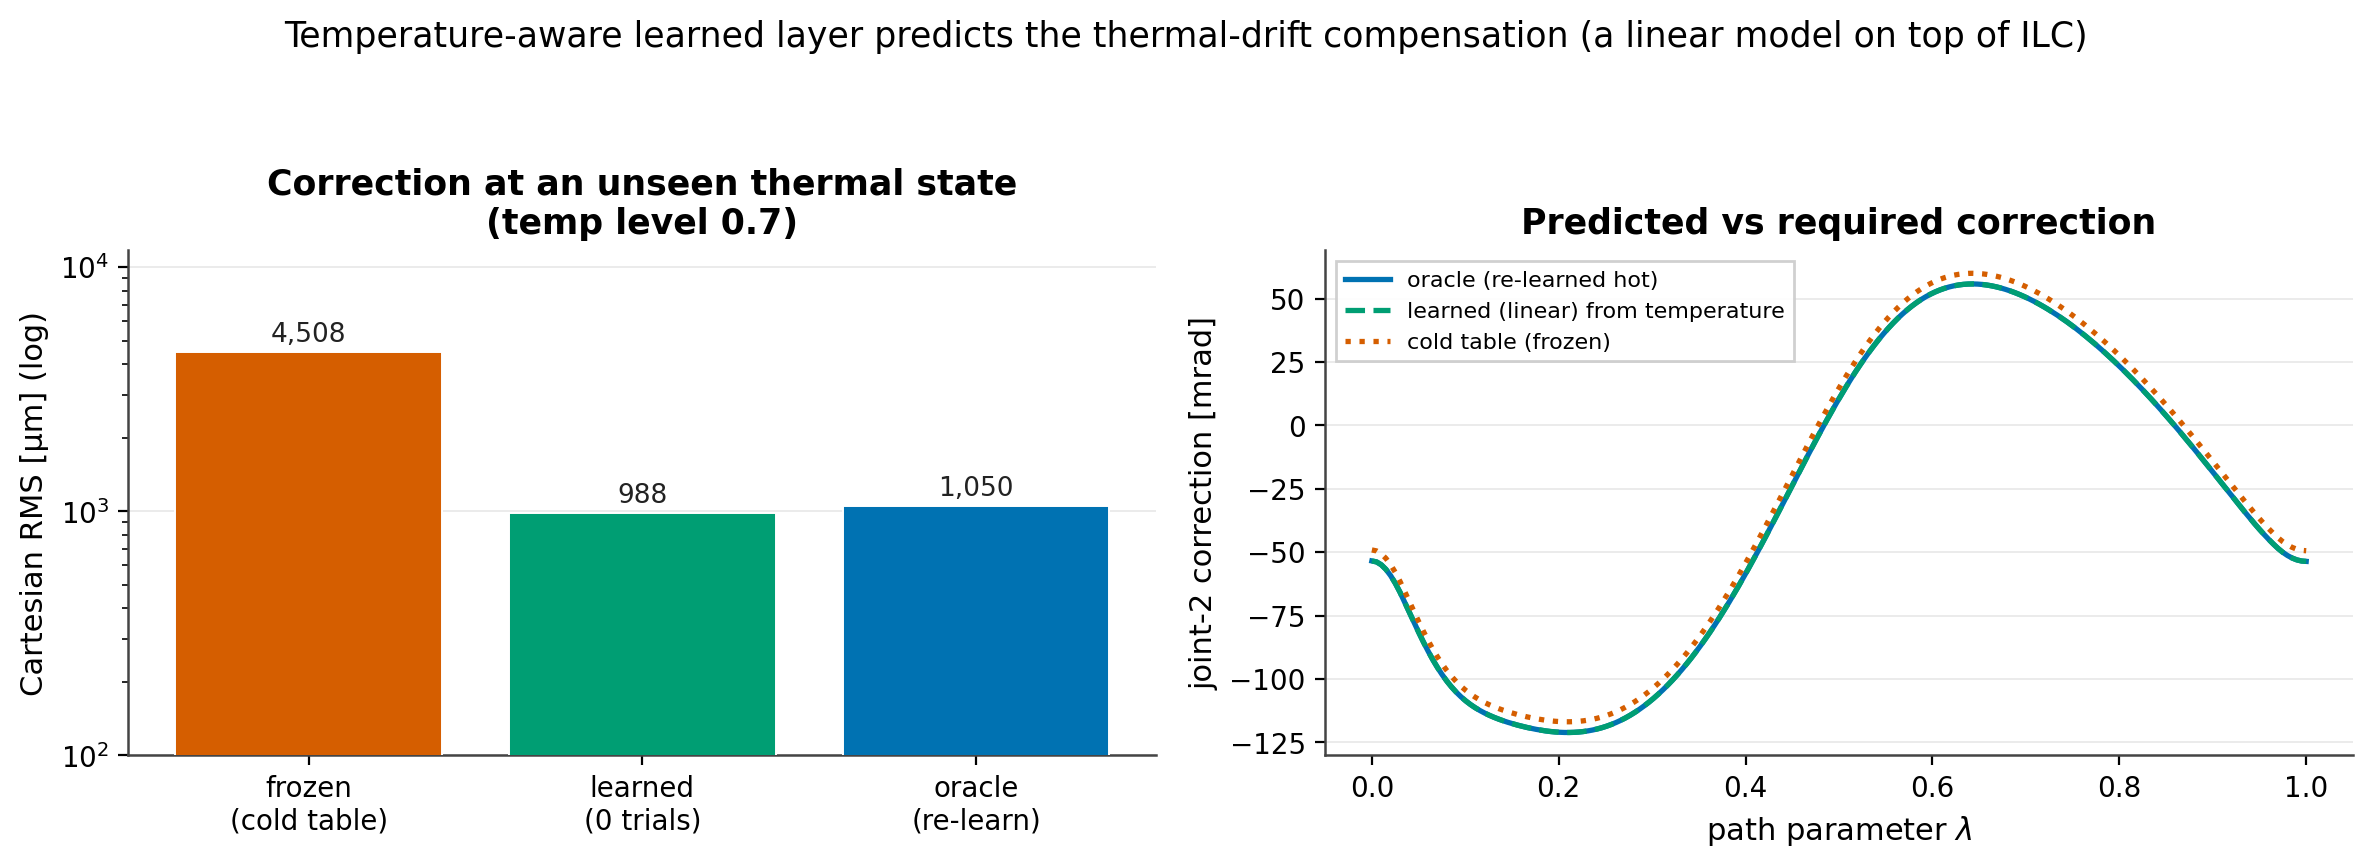
\includegraphics[width=\linewidth]{../outputs/thermal_learned_compensation.png}\\{\footnotesize (c) learned, unseen thermal state}\end{minipage}
  \caption{Headline results: (a) ILC convergence from the joint-side encoder only;
  (b) the neural-network layer on an unseen path, zero trials; (c) the
  temperature-aware learned layer at an unseen thermal state.}
  \label{fig:headline}
\end{figure*}

\textbf{Self-learning without a tracker.} Using only the joint-side encoder, the
ILC drives the tool error from $34$\,mm to ${\approx}1.06$\,mm in 2--3 trials
(${\sim}32\times$). A validation experiment (Fig.~\ref{fig:gallery}(b)) shows the
encoder RMS and the true TCP RMS fall in lock-step (correlation $0.97$),
confirming the encoder is a faithful proxy for absolute accuracy.

\textbf{Generalization to a new path.} Reusing a table learned on path A barely
helps on a different path B ($42\to14$\,mm); a full re-learn works but costs trials
($1.66$\,mm). The learned layer predicts a correction for an unseen path and
reaches $1.46$\,mm with \emph{zero} trials.

\textbf{Thermal drift.} Thermal drift is non-repetitive, so a frozen table degrades
as the robot warms ($1.0\to2.3$\,mm); an online ILC tracks it
(Fig.~\ref{fig:gallery}(h)). A temperature-aware layer predicts the compensation
at an unseen thermal state and reaches $0.99$\,mm, matching an oracle re-learn
($1.05$\,mm).

\textbf{Other KUKA experiments.} Fig.~\ref{fig:kuka} shows speed transfer (best at
the trained speed; partial elsewhere---the paper's open speed-variation issue),
path transfer without the learned layer, and a \emph{contact} task in which the
tool is dragged on a worktable under a ${\sim}108$\,N press: the same ILC reduces
the in-plane error by ${\sim}17\times$.

\begin{figure*}[t]
  \centering
  \begin{minipage}{0.32\textwidth}\centering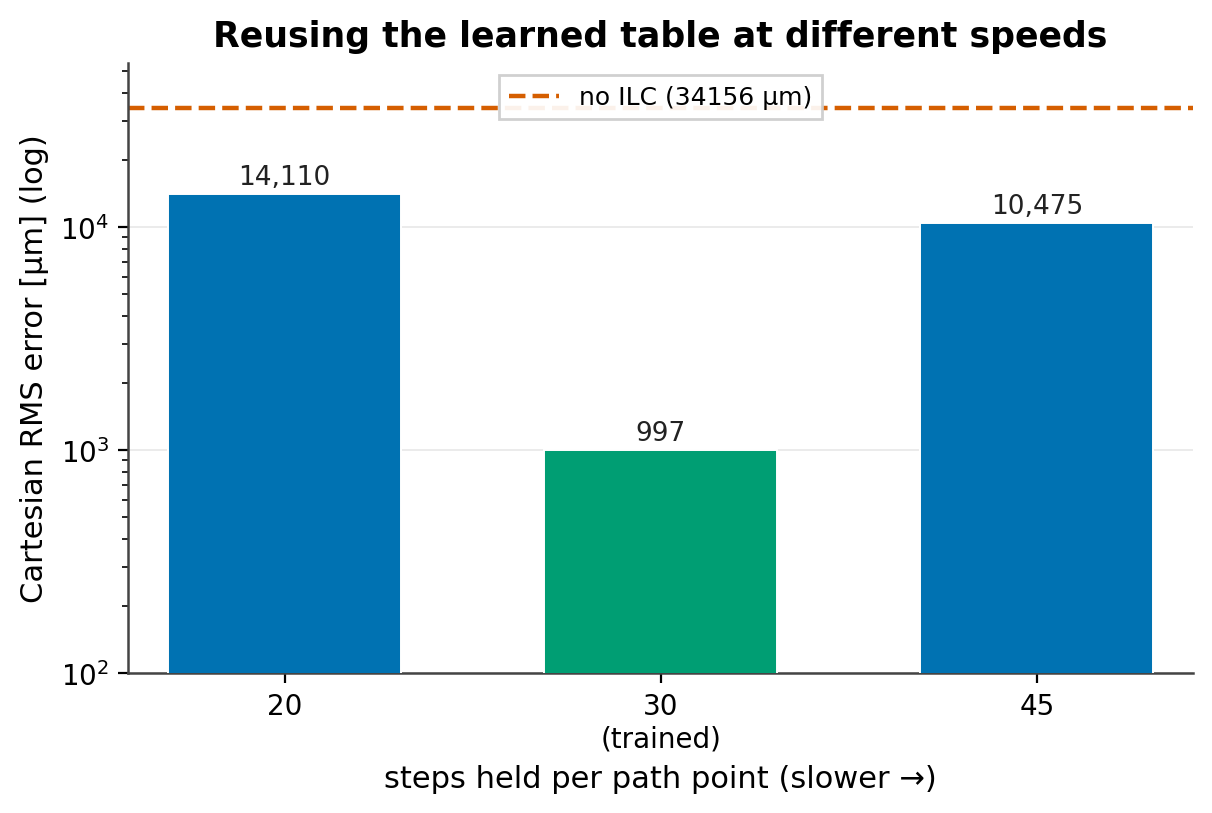
\includegraphics[width=\linewidth]{../outputs/kuka_speed_generalization.png}\\{\footnotesize (a) speed transfer}\end{minipage}\hfill
  \begin{minipage}{0.32\textwidth}\centering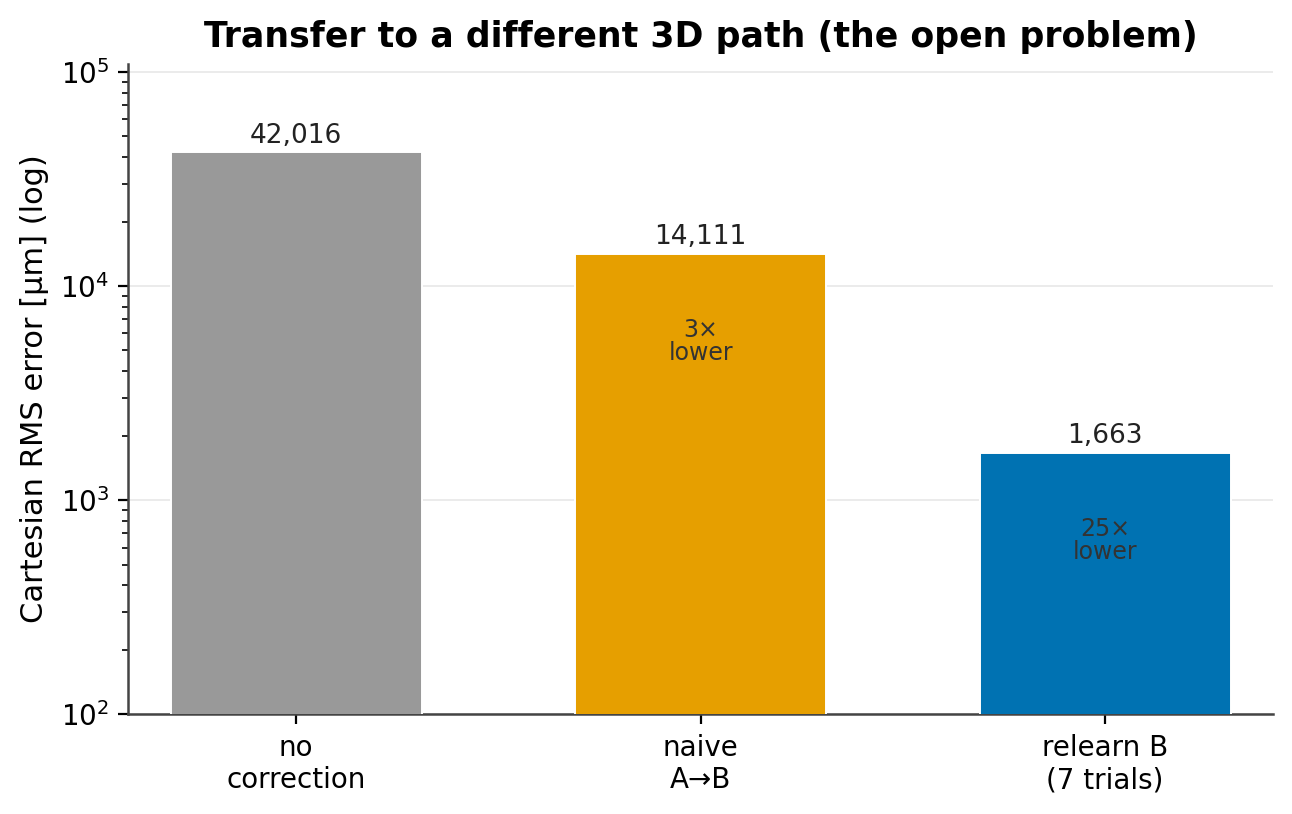
\includegraphics[width=\linewidth]{../outputs/kuka_path_transfer.png}\\{\footnotesize (b) path transfer (no learned layer)}\end{minipage}\hfill
  \begin{minipage}{0.32\textwidth}\centering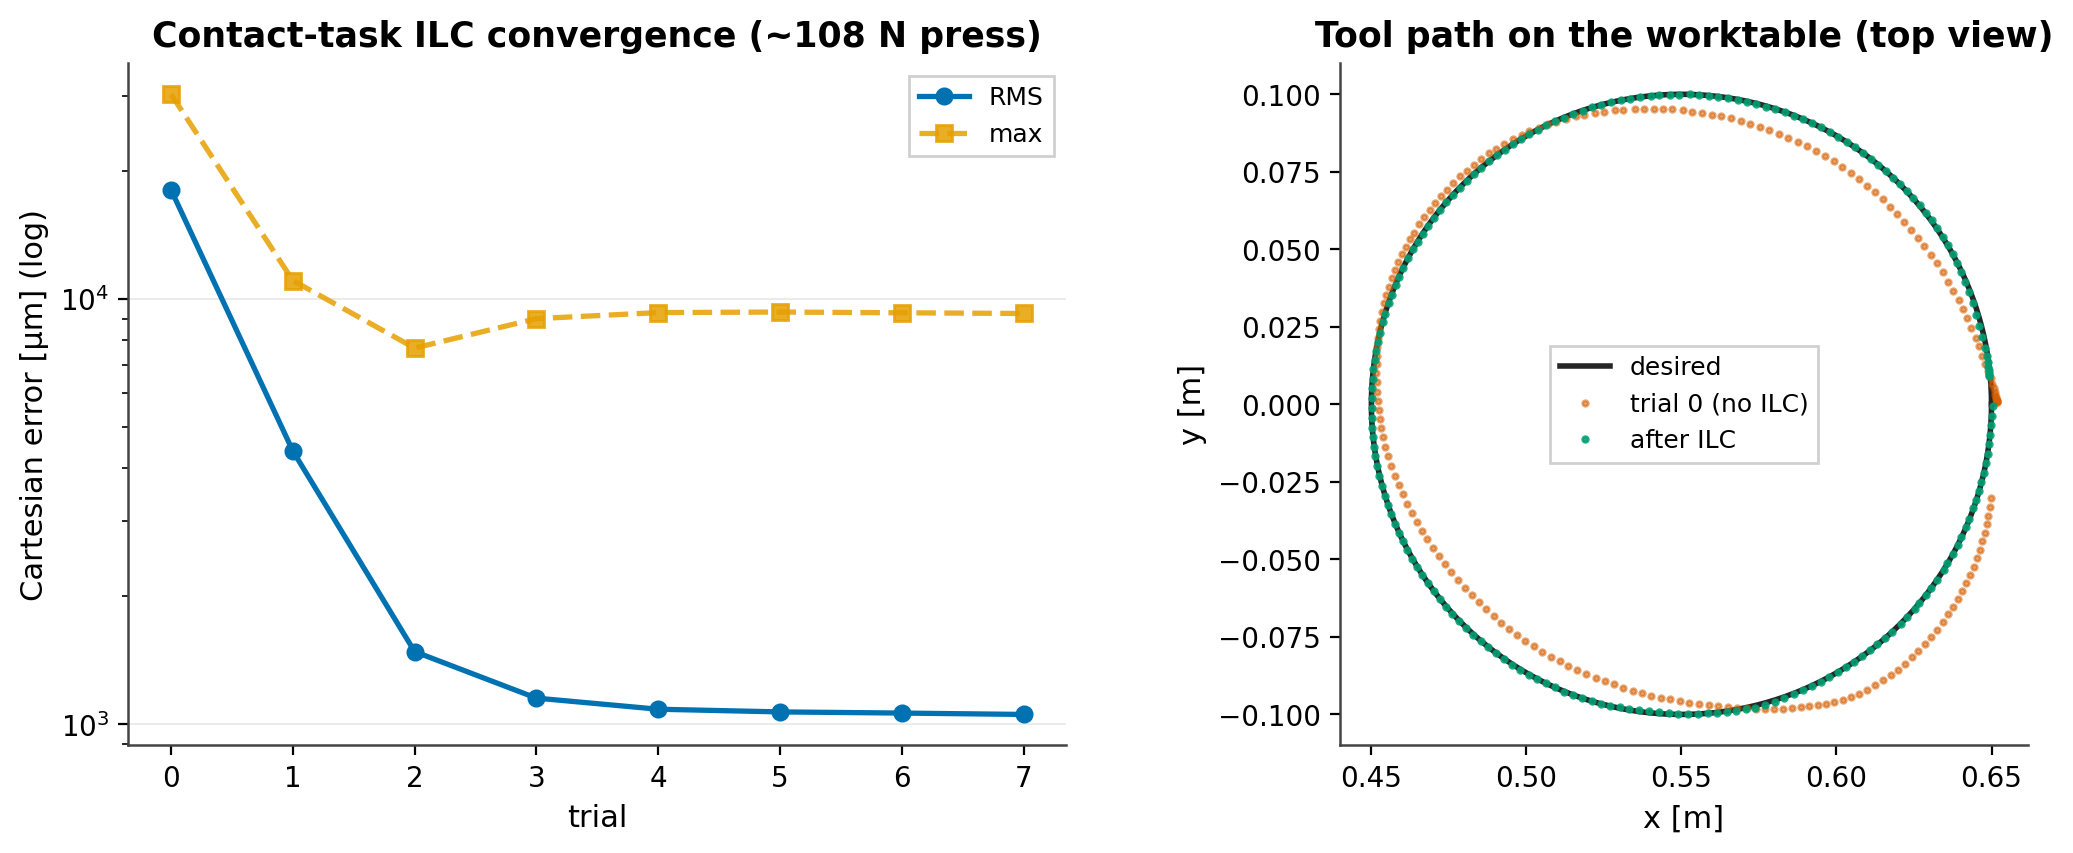
\includegraphics[width=\linewidth]{../outputs/kuka_contact_task.png}\\{\footnotesize (c) contact task, ${\sim}108$\,N}\end{minipage}
  \caption{Further KUKA experiments: (a) reusing the table at other speeds;
  (b) path A$\to$B transfer without the learned layer; (c) ILC on a tool pressed on
  a worktable.}
  \label{fig:kuka}
\end{figure*}

\textbf{Detailed analysis.} Fig.~\ref{fig:gallery} collects the supporting
figures: (a) the paper's trial-wise plot and (b) the no-tracker validation;
(c) the error along the path and (d) the spring--mass--damper view of the
joints; and (e)--(h) an ablation isolating each realistic effect---the ILC
stays ${\sim}1$\,mm under all of them, the Q-filter rejects encoder noise, and the
injected transmission error and thermal drift behave as modeled.

\begin{figure*}[t]
  \centering
  \begin{minipage}{0.245\textwidth}\centering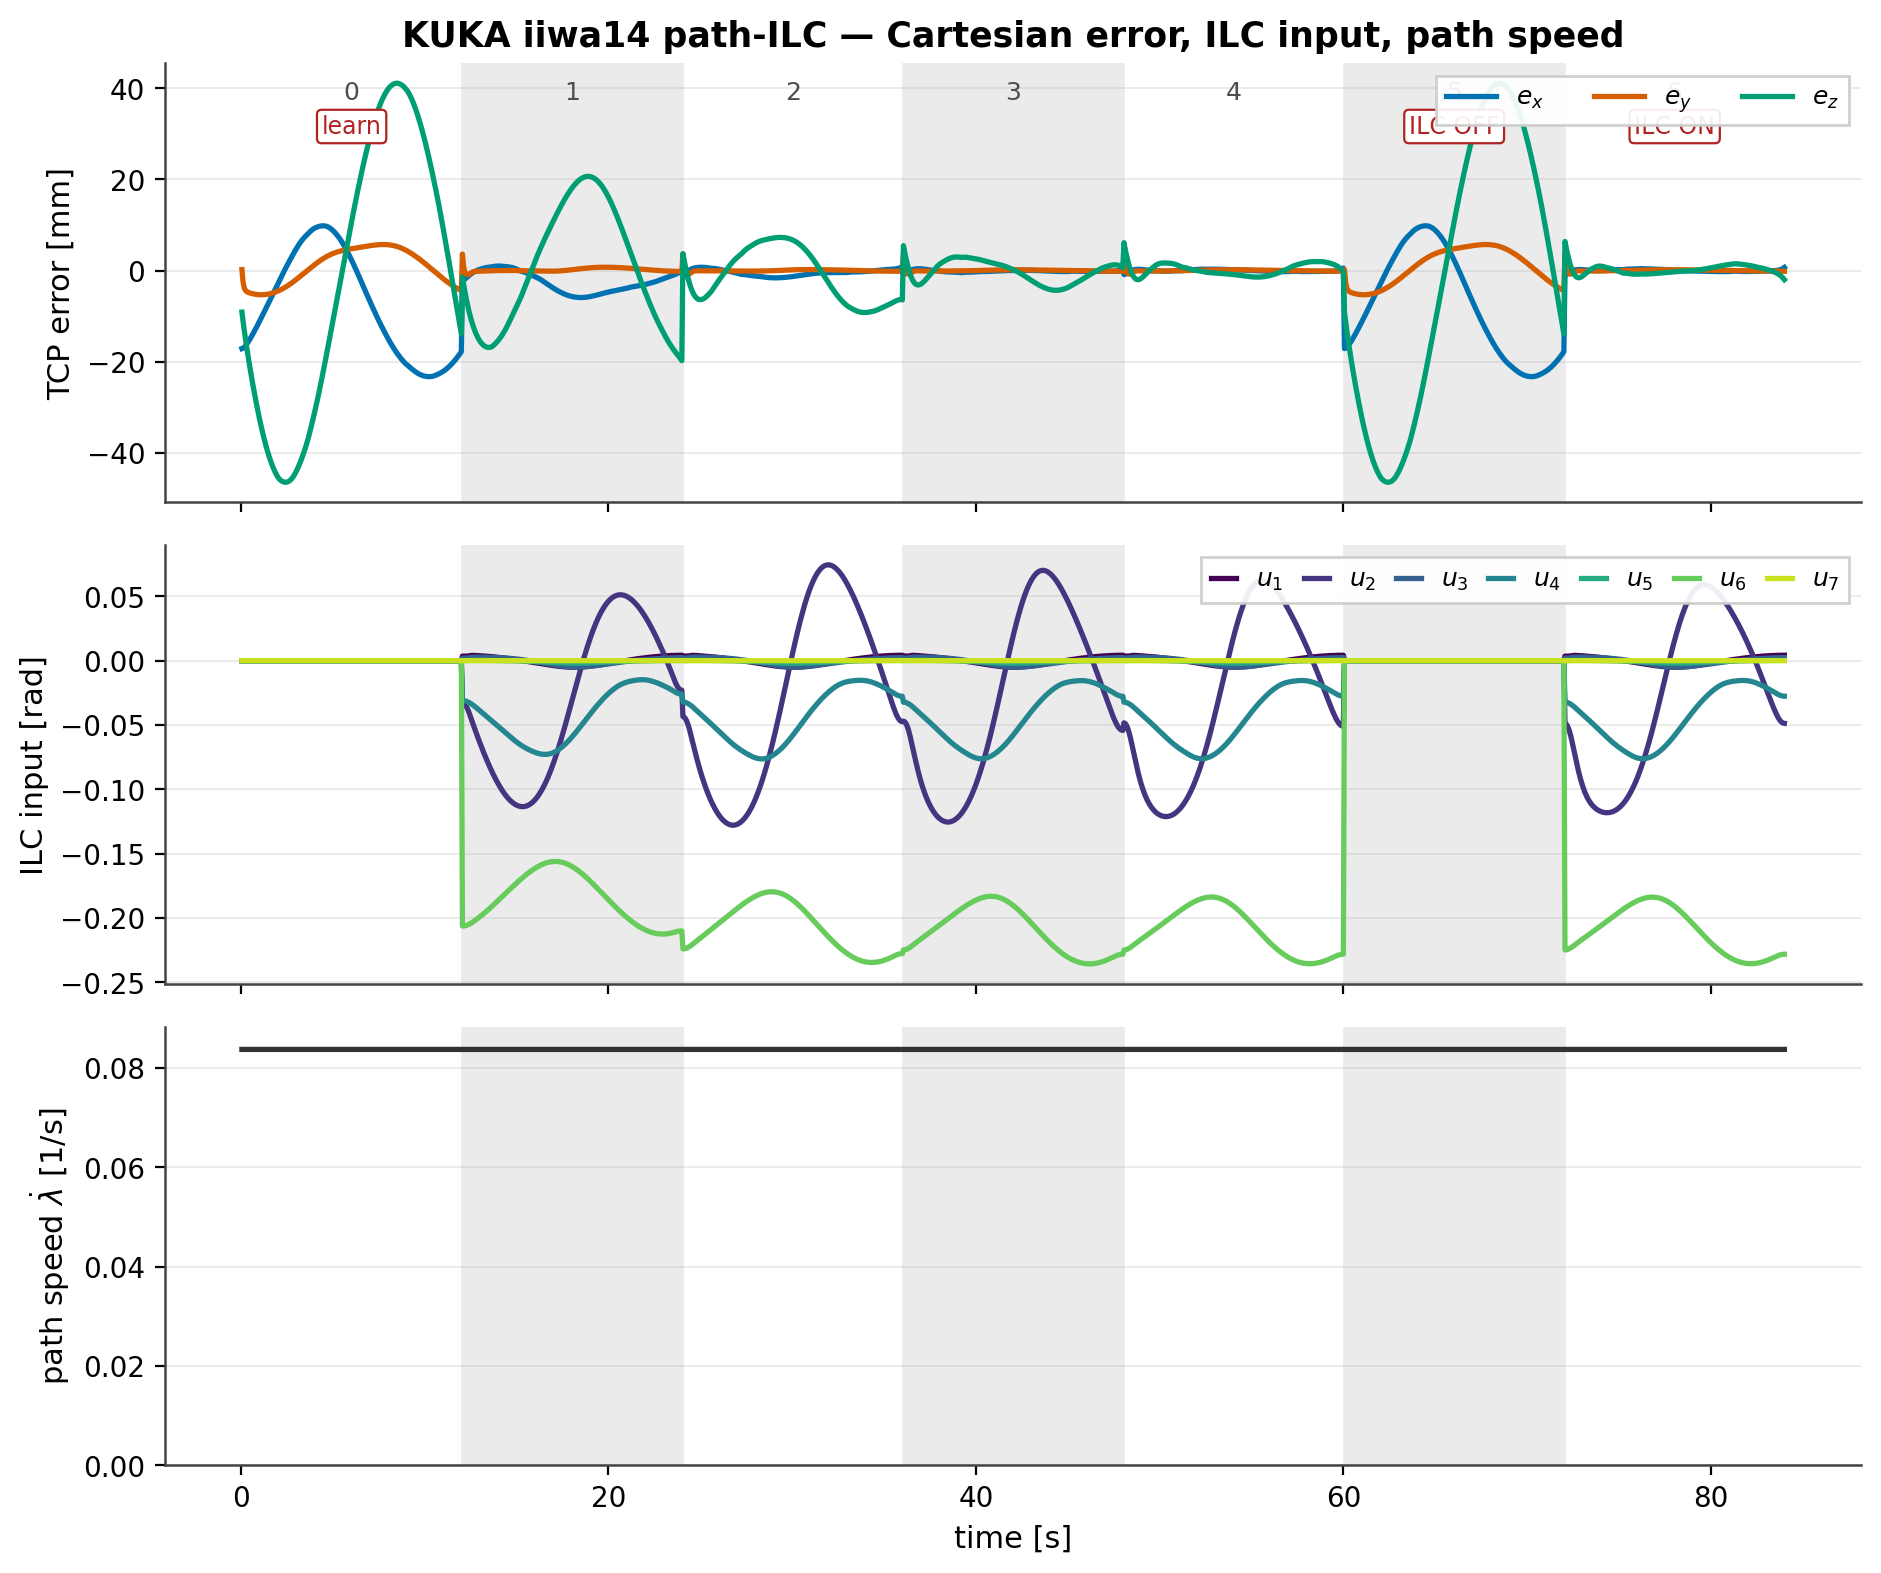
\includegraphics[width=\linewidth]{../outputs/trialwise_overview.png}\\{\footnotesize (a) paper Fig.\,5 reproduction}\end{minipage}\hfill
  \begin{minipage}{0.245\textwidth}\centering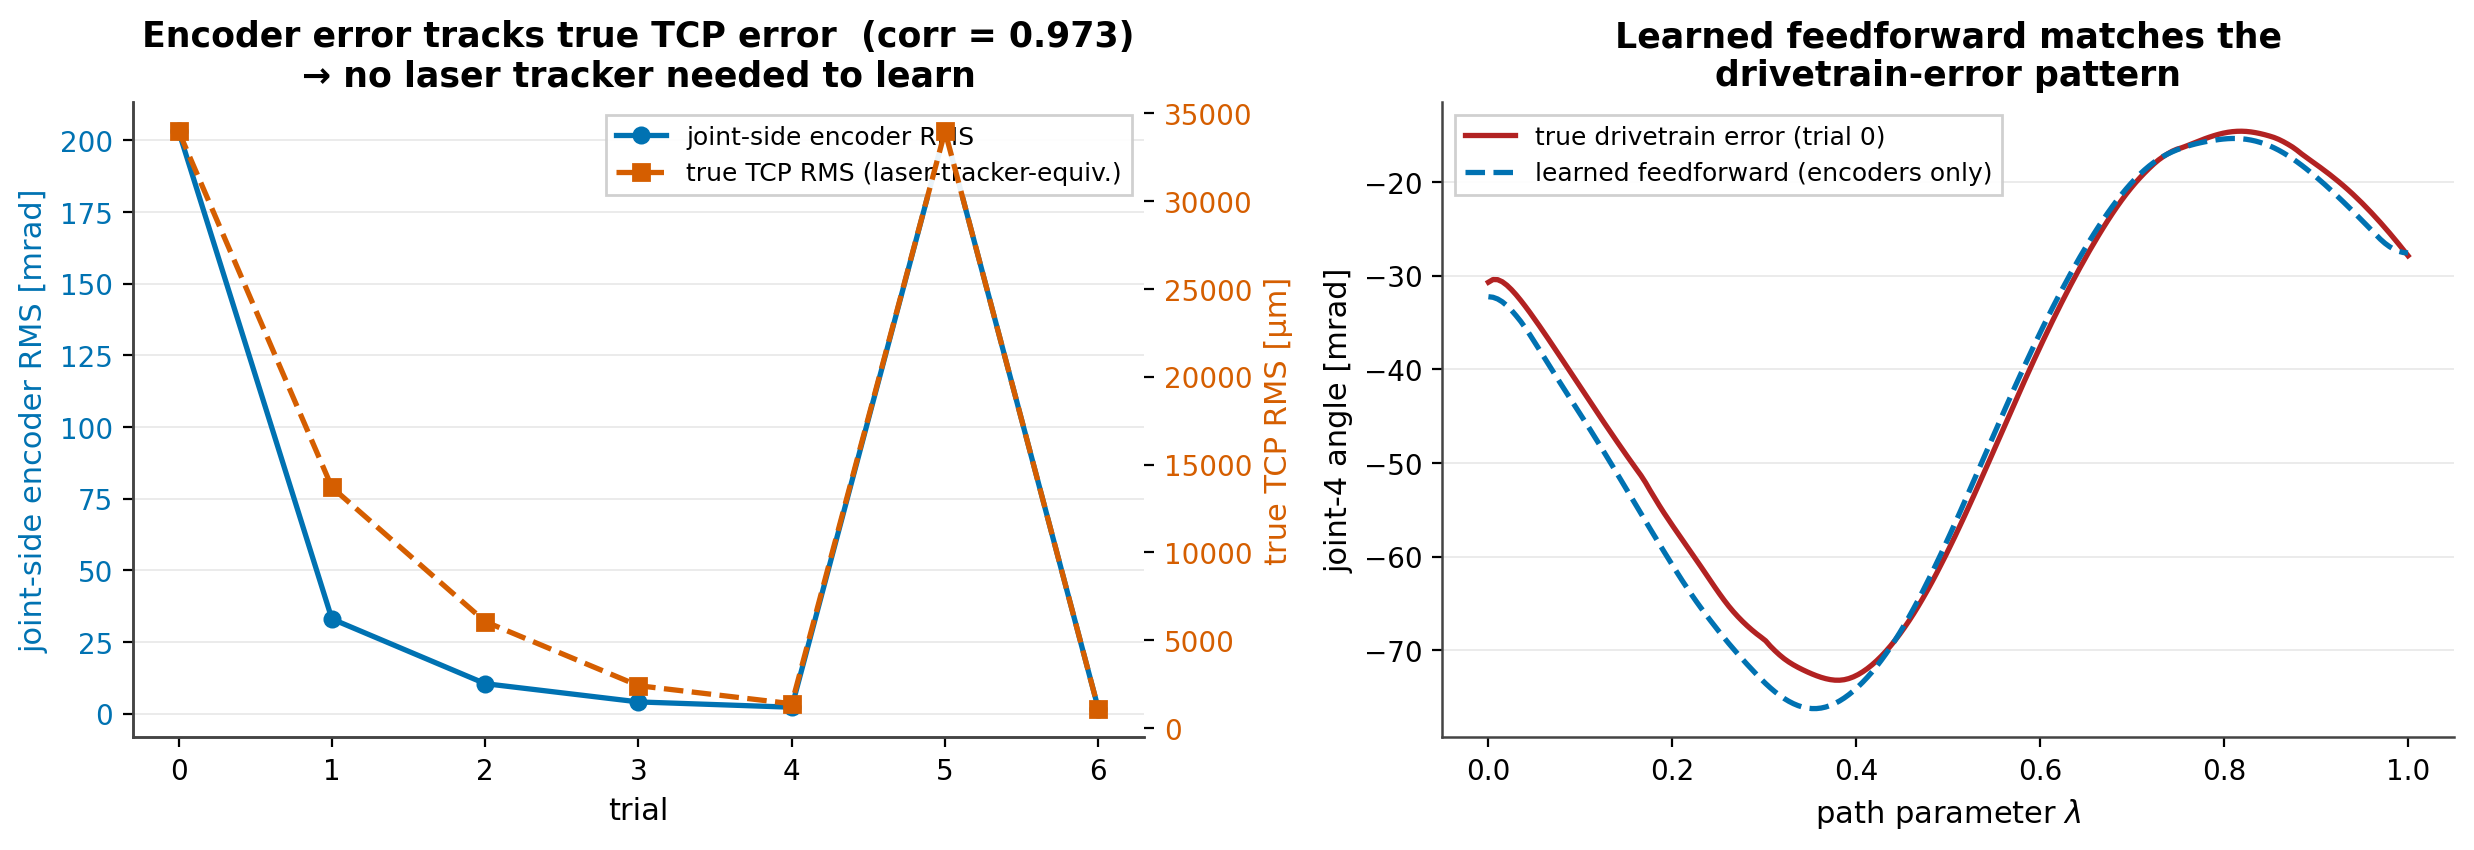
\includegraphics[width=\linewidth]{../outputs/encoder_validation.png}\\{\footnotesize (b) no-tracker validation (corr 0.97)}\end{minipage}\hfill
  \begin{minipage}{0.245\textwidth}\centering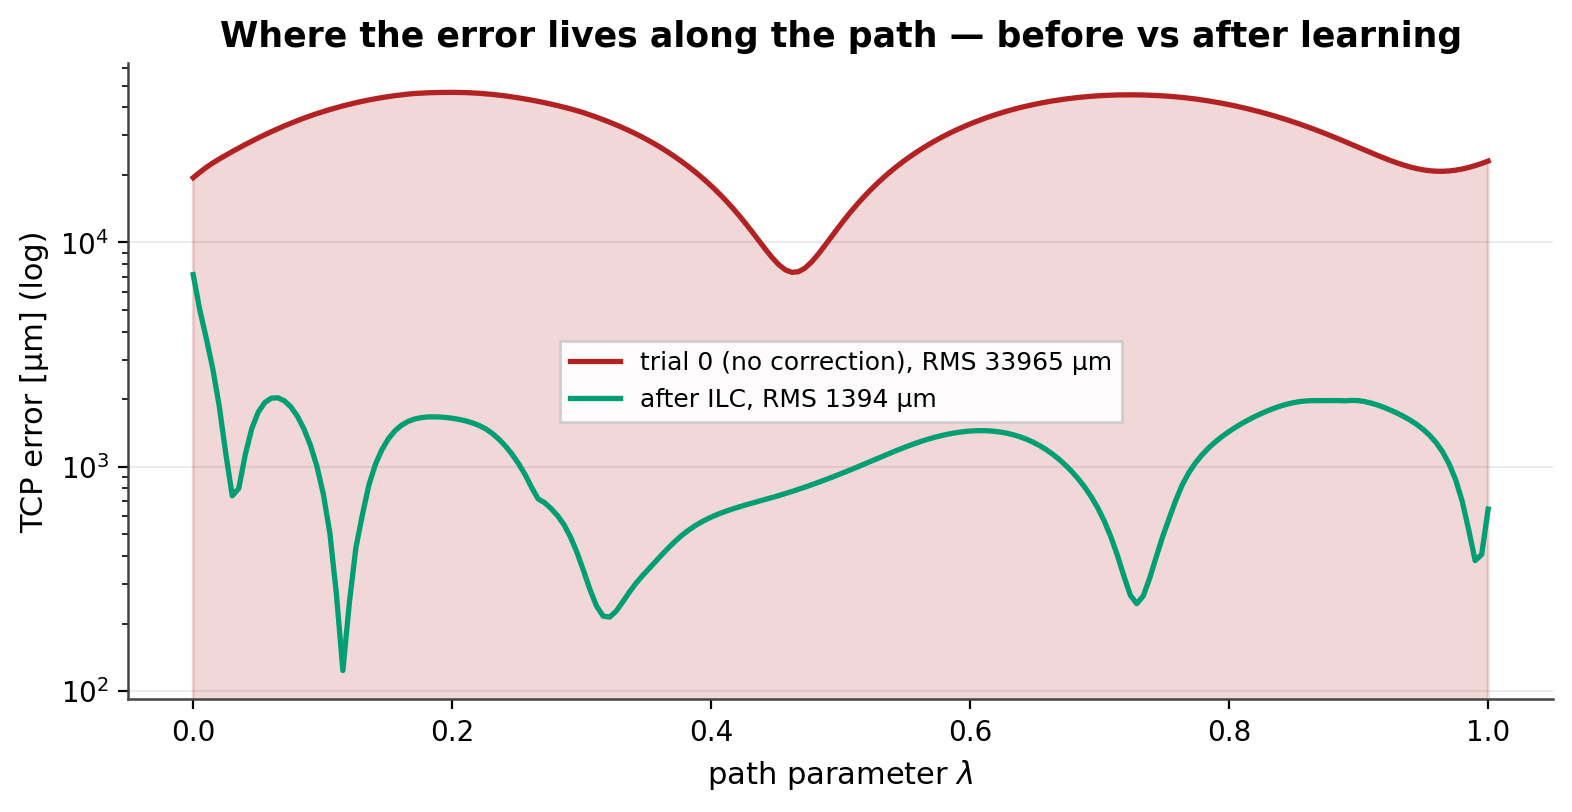
\includegraphics[width=\linewidth]{../outputs/error_along_path.png}\\{\footnotesize (c) error along the path}\end{minipage}\hfill
  \begin{minipage}{0.245\textwidth}\centering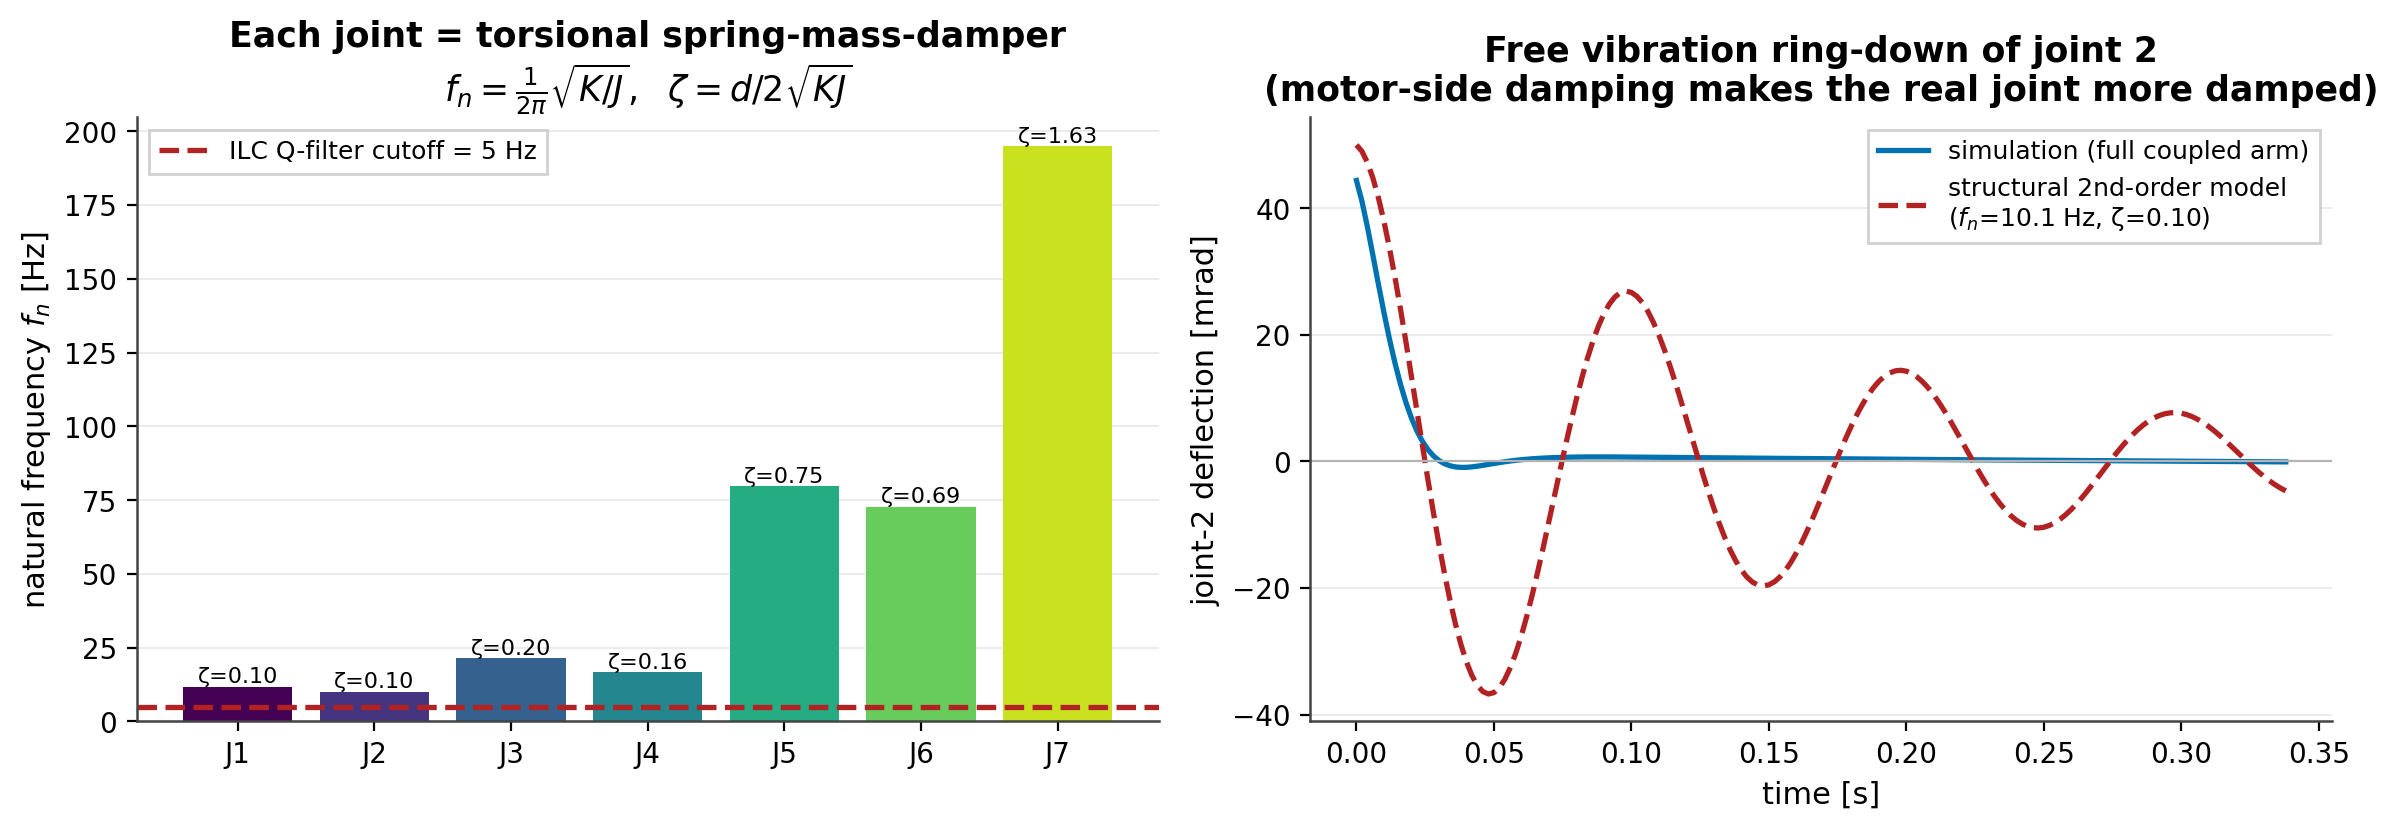
\includegraphics[width=\linewidth]{../outputs/joint_modal_properties.png}\\{\footnotesize (d) joint spring-mass-damper}\end{minipage}\\[3mm]
  \begin{minipage}{0.245\textwidth}\centering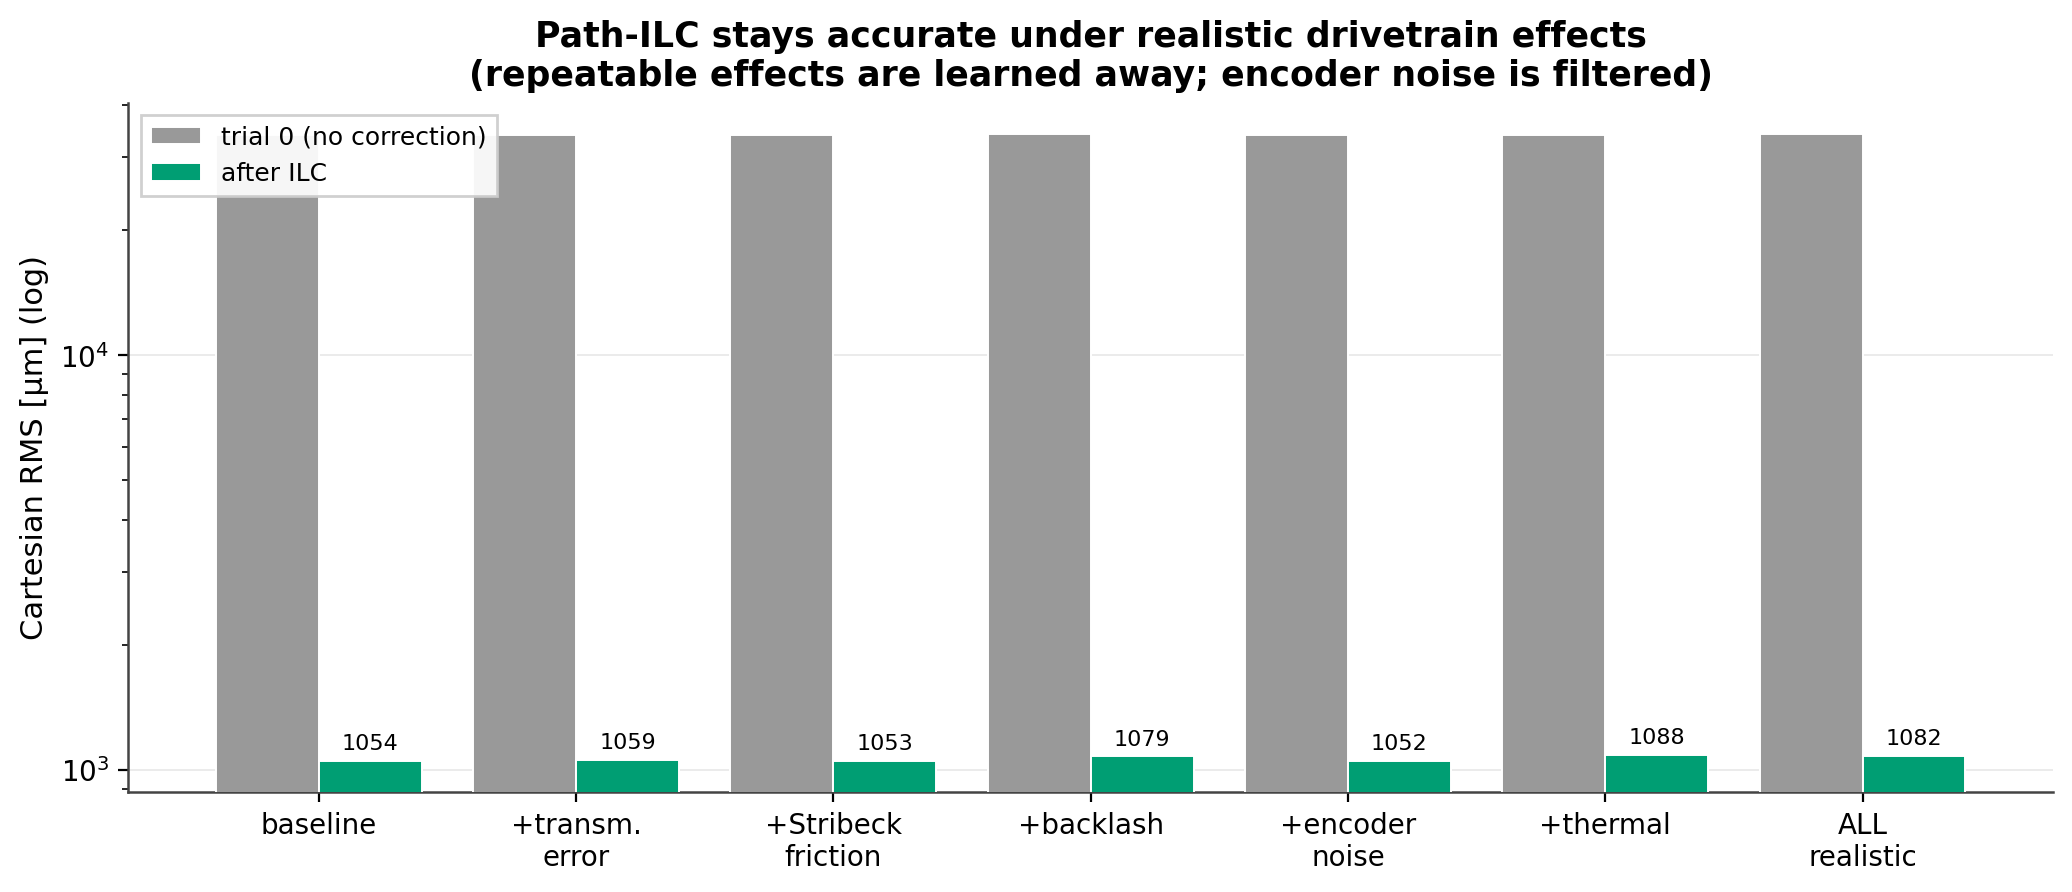
\includegraphics[width=\linewidth]{../outputs/realistic_effects_ablation.png}\\{\footnotesize (e) ablation across effects}\end{minipage}\hfill
  \begin{minipage}{0.245\textwidth}\centering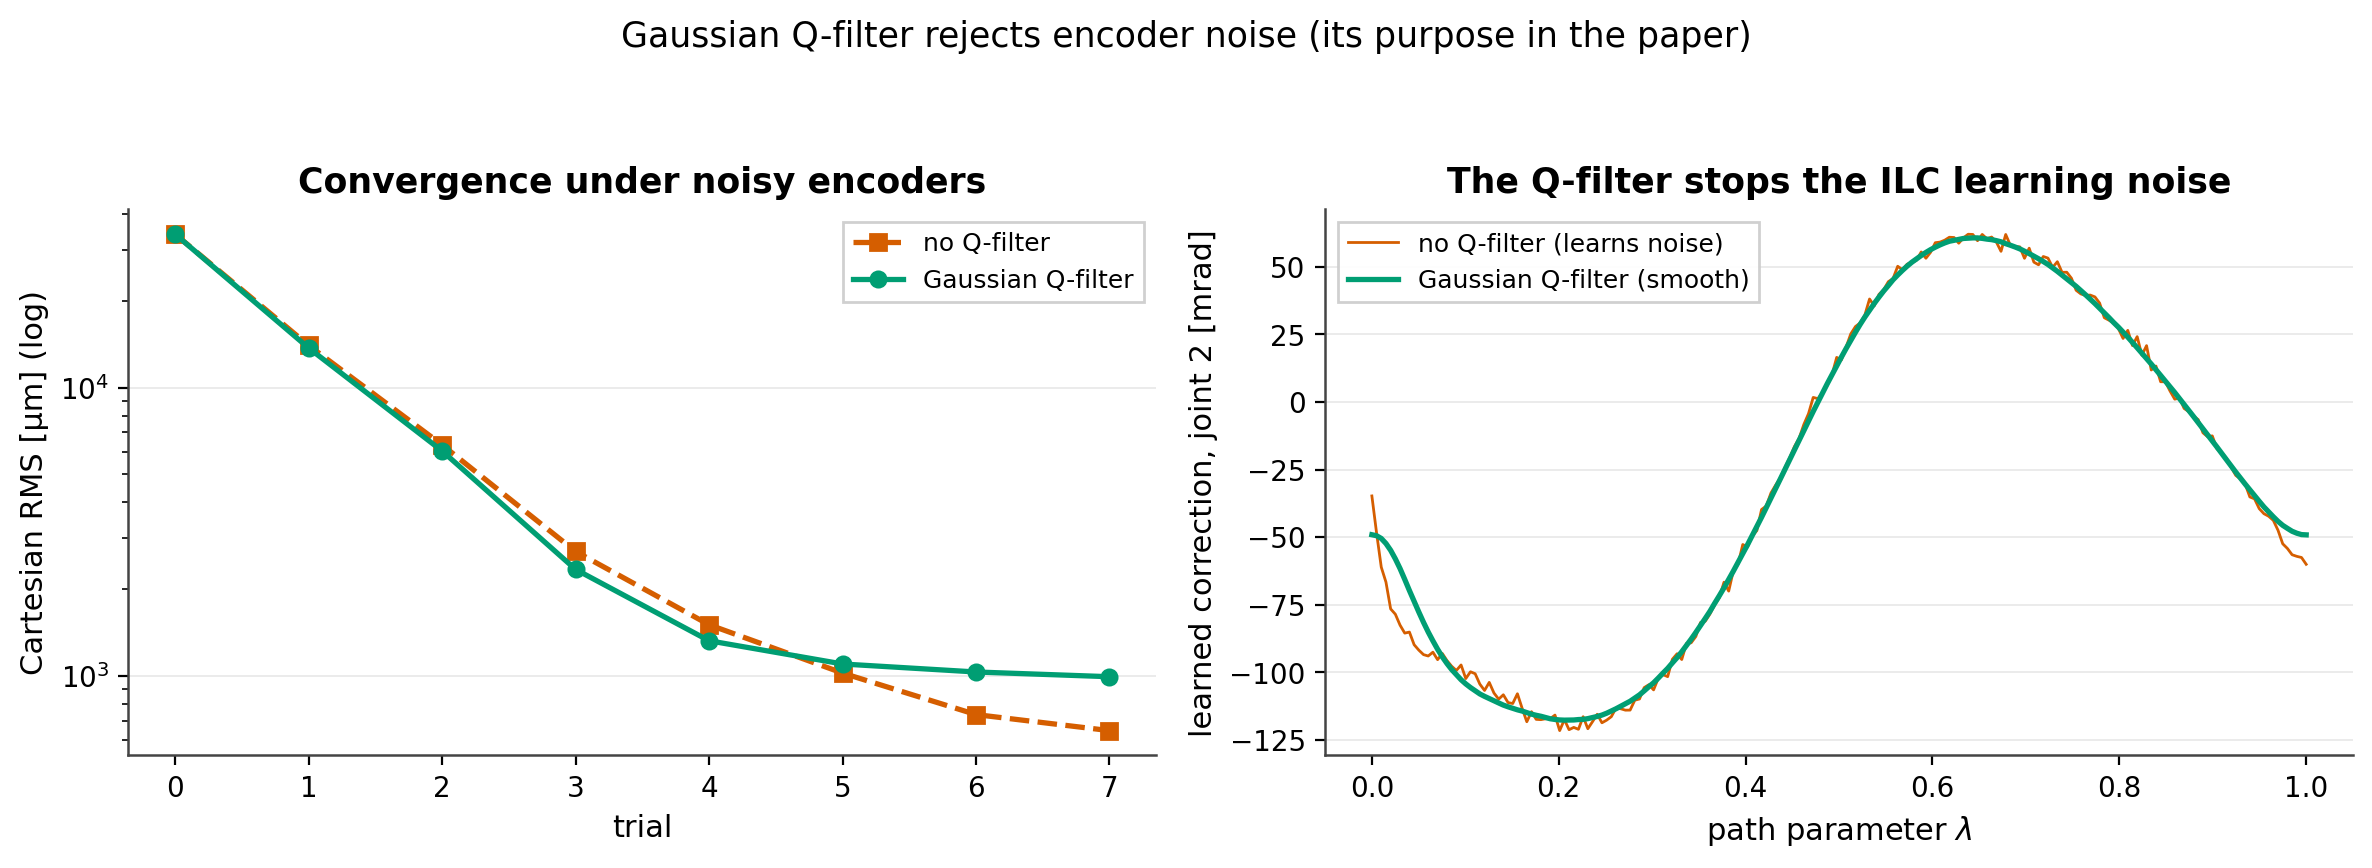
\includegraphics[width=\linewidth]{../outputs/qfilter_noise_rejection.png}\\{\footnotesize (f) Q-filter noise rejection}\end{minipage}\hfill
  \begin{minipage}{0.245\textwidth}\centering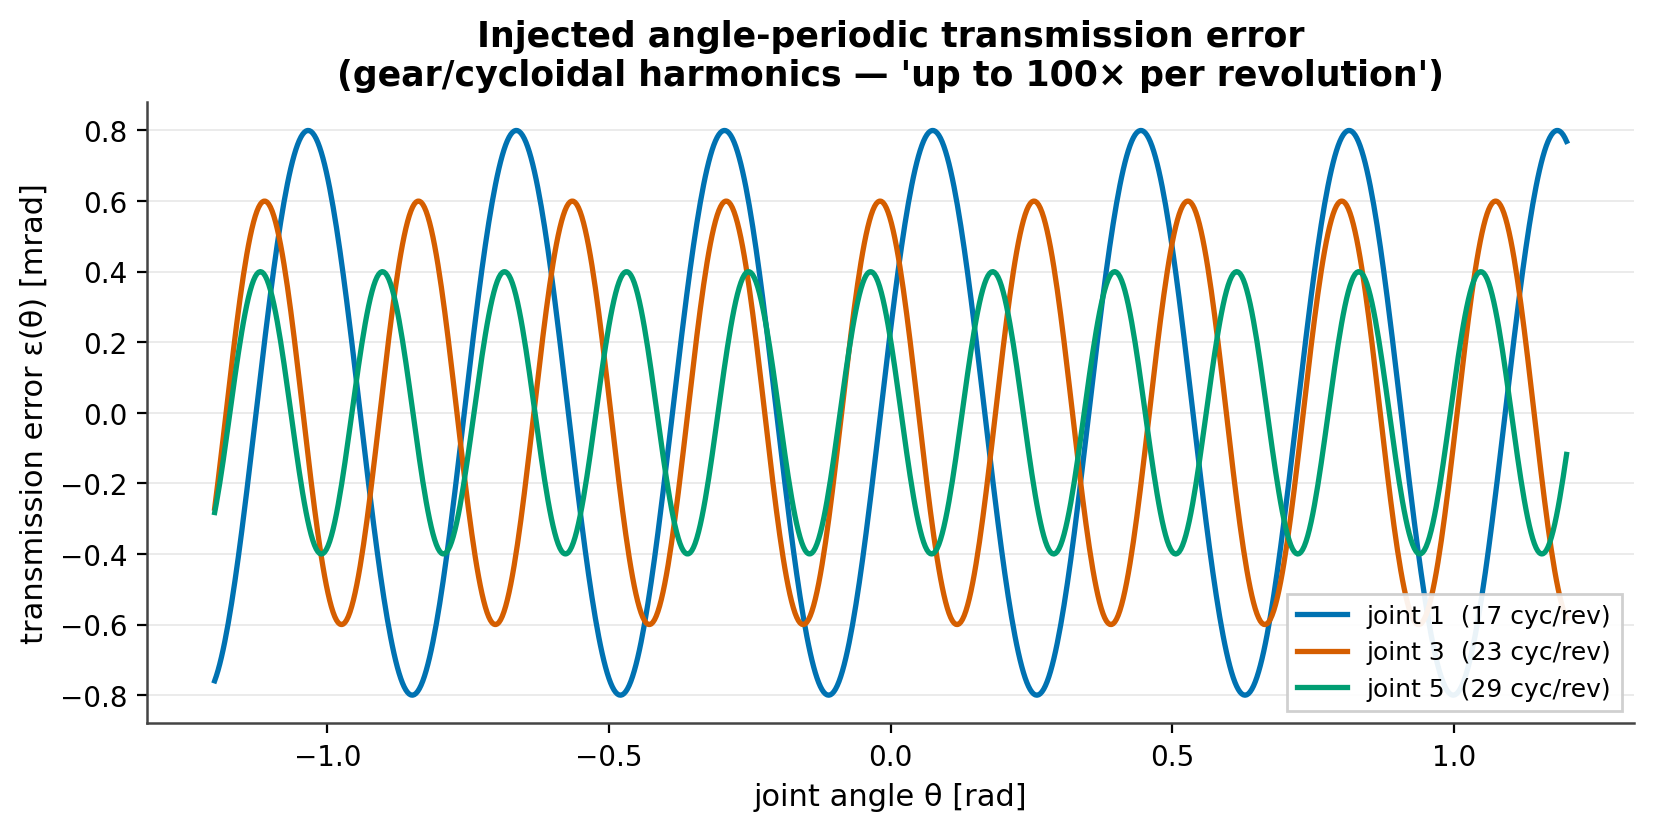
\includegraphics[width=\linewidth]{../outputs/transmission_error_profile.png}\\{\footnotesize (g) injected transmission error}\end{minipage}\hfill
  \begin{minipage}{0.245\textwidth}\centering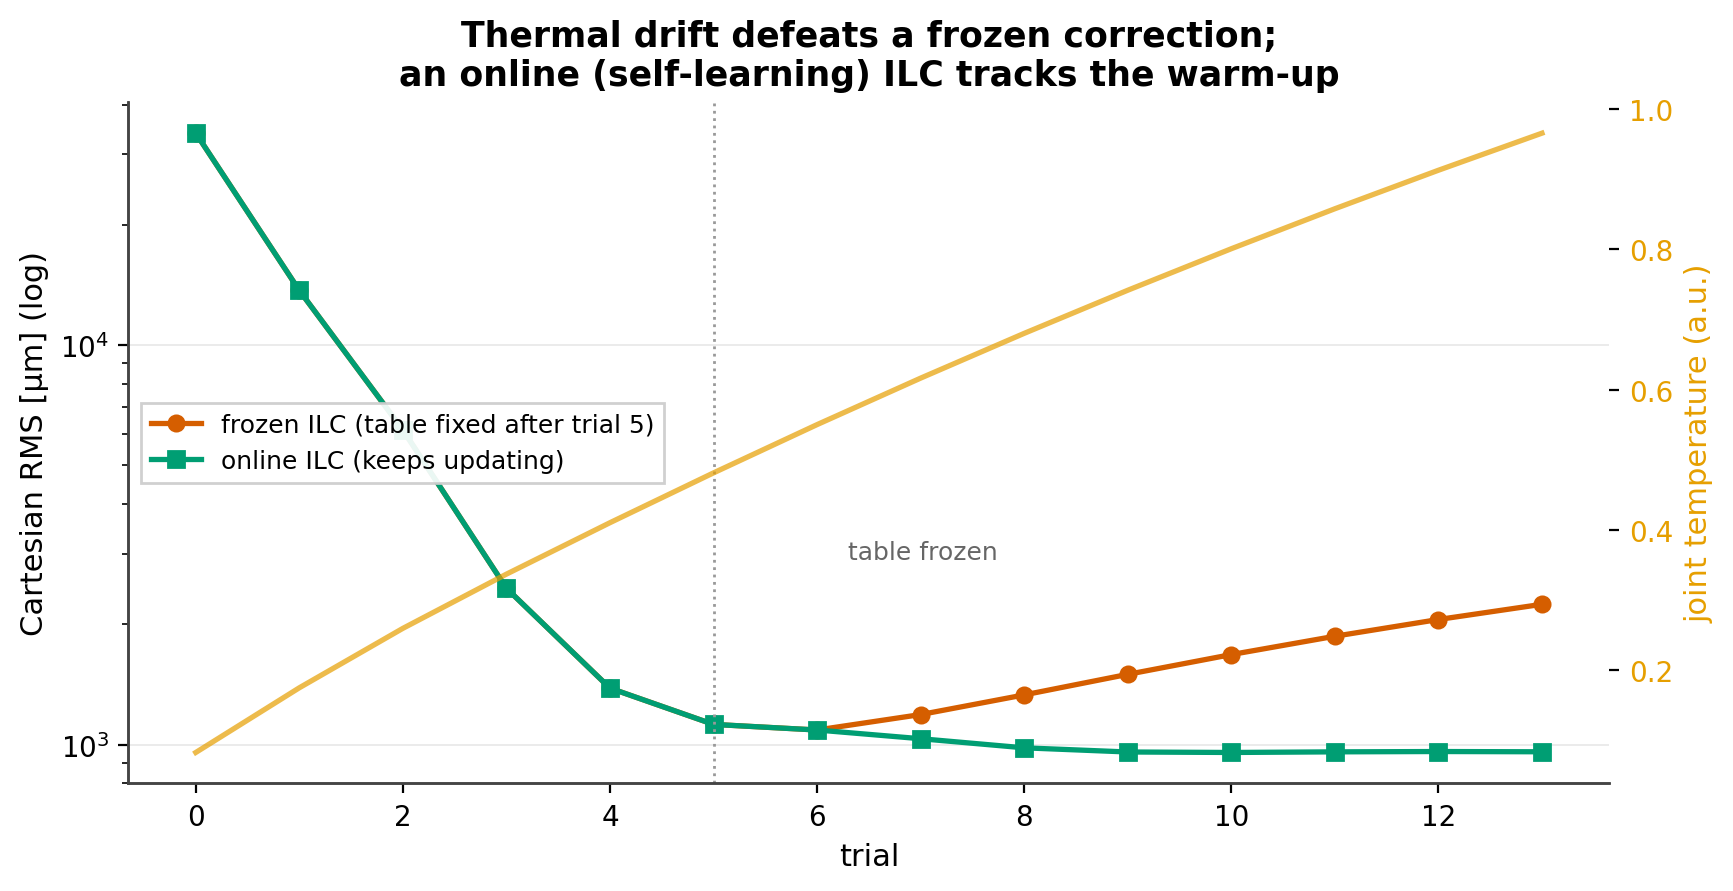
\includegraphics[width=\linewidth]{../outputs/thermal_frozen_vs_online.png}\\{\footnotesize (h) thermal: frozen vs online}\end{minipage}
  \caption{Analysis (a--d) and realistic-effect (e--h) figures. (a) trial-wise error / ILC inputs / path speed (trial 5 ILC-off, 6 on); (b) encoder RMS vs true TCP RMS in lock-step; (c) where the error lives along the path; (d) joint natural frequencies vs the Q-filter cutoff; (e) ILC stays ${\sim}1$\,mm under every effect; (f) Q-filter noise rejection; (g) the injected angle-periodic transmission error; (h) thermal drift defeats a frozen table while an online ILC tracks it.}
  \label{fig:gallery}
\end{figure*}

\section{Discussion: Honest Scope}\label{sec:disc}
This is a simulation, and two points deserve emphasis. First, the sensing
assumption is \emph{stronger} than the original hardware: our joint-side encoder
reads the true link angle and thus \emph{directly} observes the drivetrain error,
whereas the laser tracker in~\cite{schwegel2024} is needed precisely because
motor-side encoders cannot. Real secondary encoders have noise and resolution
limits, and a joint-to-task kinematic-calibration gap remains that a joint sensor
cannot see. Second, speed transfer is only partial: a position-indexed table
cannot cancel a velocity-dependent residual, an effect enlarged by our position
controller relative to the paper's computed-torque scheme. The learned layer is
also an easy instance here (smooth low-dimensional paths); the contribution is the
\emph{architecture and protocol}---train on real ILC-solved tables, test on an
unseen case---rather than the difficulty of this instance. Third, the gains are
the paper's defaults applied uniformly; a mild per-axis schedule (a higher $K_p$
on the stiff wrist joints) would likely trim the residual further, so the absolute
micrometre figures should be read as representative rather than optimized.

What would it take on hardware? The pieces map cleanly onto a real cell. The
joint-side encoder is the secondary encoder that high-accuracy arms increasingly
carry; the path-parameter table and Gaussian Q-filter are a few lines of
feedforward around the existing position loop; and the learned layer trains
entirely offline, from tables the robot produces during its own ILC runs, so no
extra instrumentation is needed at deployment. The risks are precisely the ones a
simulation hides: finite encoder resolution and noise, the kinematic-calibration
gap between joint space and task space that an output encoder cannot observe, and
load- or temperature-dependent dynamics richer than our two-mass model. That is
why we frame the result as an \emph{architecture} validated in simulation rather
than a deployment claim---each open problem above is a concrete next experiment,
not a hidden assumption.

Finally, a word on cost and division of labour. Nothing here is expensive at run
time: the ILC update is one filtered PD pass per arc-length sample, and the
learned layer is a single forward evaluation of a small network, both negligible
beside the physics step. The design deliberately keeps the \emph{repeatable},
structured part of the error with the classical ILC---where it is interpretable
and provably convergent---and asks the network only to \emph{interpolate between
converged solutions} across contexts. That separation is why the learned layer can
stay small and why a failure is diagnosable: if the prediction is poor on a new
path, a few ordinary ILC trials recover it and simultaneously become fresh
training data. The friction, transmission-error and thermal models we inject are
standard ones~\cite{armstrong1994,litak2003}, so the difficulty the ILC faces is
representative rather than adversarial.

\section{Conclusion}
We re-implemented a path-parameter ILC on a physically detailed flexible-joint
KUKA iiwa14~\cite{spong1987} and extended it toward three of its stated open
problems: tracker-free self-learning from a joint-side encoder, zero-trial
generalization to new paths via a small neural network, and compensation of
non-repetitive thermal drift with a temperature-indexed model. Across all of them
the tool error stays near $1$\,mm, the limitations are stated plainly, and the
methods are released as a single reproducible pipeline. The natural next step is
hardware: a real secondary encoder, a kinematic-calibration stage to close the
joint-to-task gap, and on-robot collection of the converged tables that train the
learned layer. We expect the classical core to transfer directly and the learned
layer to need richer context features (load, pose, temperature) than the smooth
paths studied here demand.

\FloatBarrier
\begin{thebibliography}{9}\small
\bibitem{schwegel2024} M.~Schwegel and A.~Kugi, ``A Simple Computationally
Efficient Path ILC for Industrial Robotic Manipulators,'' in \emph{Proc. IEEE
ICRA}, 2024, pp.~2133--2139.
\href{https://doi.org/10.1109/ICRA57147.2024.10610623}{\texttt{doi:10.1109/ICRA57147.2024.10610623}}
\bibitem{bristow2006} D.~A.~Bristow, M.~Tharayil, and A.~G.~Alleyne, ``A survey of
iterative learning control,'' \emph{IEEE Control Syst. Mag.}, vol.~26, no.~3,
pp.~96--114, 2006.
\href{https://doi.org/10.1109/MCS.2006.1636313}{\texttt{doi:10.1109/MCS.2006.1636313}}
\bibitem{litak2003} G.~Litak and M.~I.~Friswell, ``Vibration in gear systems,''
\emph{Chaos, Solitons \& Fractals}, vol.~16, no.~5, pp.~795--800, 2003.
\href{https://doi.org/10.1016/S0960-0779(02)00452-6}{\texttt{doi:10.1016/S0960-0779(02)00452-6}}
\bibitem{spong1987} M.~W.~Spong, ``Modeling and control of elastic joint robots,''
\emph{ASME J. Dyn. Syst. Meas. Control}, vol.~109, no.~4, pp.~310--319, 1987.
\href{https://doi.org/10.1115/1.3143860}{\texttt{doi:10.1115/1.3143860}}
\bibitem{armstrong1994} B.~Armstrong-H\'elouvry, P.~Dupont, and C.~Canudas de Wit,
``A survey of models, analysis tools and compensation methods for the control of
machines with friction,'' \emph{Automatica}, vol.~30, no.~7, pp.~1083--1138, 1994.
\href{https://doi.org/10.1016/0005-1098(94)90209-7}{\texttt{doi:10.1016/0005-1098(94)90209-7}}
\bibitem{mujoco} E.~Todorov, T.~Erez, and Y.~Tassa, ``MuJoCo: A physics engine for
model-based control,'' in \emph{Proc. IEEE/RSJ IROS}, 2012, pp.~5026--5033.
\href{https://doi.org/10.1109/IROS.2012.6386109}{\texttt{doi:10.1109/IROS.2012.6386109}}
\bibitem{menagerie} Google DeepMind, ``MuJoCo Menagerie,'' 2022. [Online].
Available: \url{https://github.com/google-deepmind/mujoco_menagerie}
\end{thebibliography}
\end{document}
